\documentclass[11pt]{article}

\usepackage[english]{babel}                 %% hyphenation rules, spell-checker
\usepackage{amsmath,amssymb}                        %% macros like align* and pmatrix
\usepackage{graphicx,epstopdf}              %% for .eps graphs
\usepackage[official]{eurosym}              %% 1 \euro
\usepackage[a4paper,margin=2cm]{geometry}   %% margins
\usepackage{hyperref}                       %% hyperlinks to urls
\usepackage{float}                    

\frenchspacing                              %% no extra space after period
\addtolength{\parskip}{0.5\baselineskip}    %% some white space between paragraphs
\setlength{\parindent}{0pt}                 %% but no indentation
\renewcommand{\baselinestretch}{1.1}        %% line spacing of TeX is small
\DeclareMathOperator{\E}{\mathbb{E}}
\DeclareMathOperator{\Var}{\text{Var}}
\DeclareMathOperator{\Cov}{\text{Cov}}


\title{Non-life --- Assignment NL3}  %% don't forget to change!

\author{
  Niels Keizer\footnote{Student number: 10910492}
  \quad and \quad
  Robert Jan Sopers\footnote{Student number: 0629049}
}

\date{\today}

\begin{document}

\maketitle

\section{GLMs and the Lee-Carter mortality model}

\subsection*{Q1}

Assuming $\beta_\Sigma := \sum \beta_x \not = 0$ and the transformation
\begin{equation}
\alpha'_x  \leftarrow \alpha_x  + \beta_x \overline{\kappa}; \quad \kappa''_t \leftarrow \kappa_t \beta_\Sigma; \quad \beta'_x \leftarrow \frac{\beta_x}{\beta_\Sigma}; \quad \kappa'_t \leftarrow \kappa''_t  - \overline{\kappa''} \quad \forall x,t
\end{equation}
a straightforward substitution of this transformation shows that 
\begin{eqnarray*}
\mu'_{xt} &=& \exp(\alpha'_x + \beta'_x \kappa'_t) \\
		  &=& \exp \left ( \alpha_x + \beta_x \bar{\kappa} + \frac{\beta_x}{\beta_\Sigma} ( \kappa''_t - \overline{\kappa''}) \right ) \\
		  &=& \exp \left (  \alpha_x + \beta_x \bar{\kappa} + \frac{\beta_x}{\beta_\Sigma} ( \kappa_t \beta_\Sigma - \overline{\kappa_t} \beta_\Sigma) \right ) \\
		  &=& \exp \left ( \alpha_x + \beta_x \bar{\kappa} + \beta_x \kappa_t - \beta_x  \bar{\kappa}\right ) = \exp(\alpha_x + \beta_x \kappa_t)  = \mu_{xt}
\end{eqnarray*}
and together with $\bar{\kappa} = \frac{1}{T} \sum_{t=1}^T \kappa_t$ we have (assuming $\beta_\Sigma \not = 0$)
\begin{equation}
\sum_x \beta'_x = \sum_x \frac{\beta_x}{\beta_\Sigma} = \frac{1}{\beta_\Sigma} \sum_x \beta_x = \frac{1}{\beta_\Sigma} \beta_\Sigma = 1
\end{equation}
and 
\begin{equation}
\sum_{t=1}^T \kappa'_t = \sum_{t=1}^T (\kappa''_t - \overline{\kappa''_t}) = \sum_{t=1}^T \kappa_t \beta_\Sigma - \sum_{t=1}^T \beta_\Sigma \overline{\kappa} = T \overline{\kappa} \beta_\Sigma - T \beta_\Sigma \overline{\kappa} =0 
\end{equation}
which are the desired properties for $\beta'_x$ and $\kappa'_t$.

\subsection*{Q2}

From (3) from the assignment we have that
\begin{equation}
\log(\mu_{xt}) = \alpha_x + \beta_x \kappa_t \Rightarrow \alpha_x = \log(\mu_{xt}) - \beta_x \kappa_t \label{question2}
\end{equation}
assuming now the property $\sum_t \kappa_t = 0$  we see that summing over $t$ gives
\begin{equation}
\sum_{t=1}^T \alpha_x = T \alpha_x = \sum_{t=1}^T \log \mu_{xt} - \beta_x \sum_{t=1}^T \kappa_t = \sum_{t=1}^T \log \mu_{xt} 
\end{equation}
which implies 
\begin{equation}
\alpha_x = \frac{1}{T} \sum_{t=1}^T \log \mu_{xt} \quad \forall x
\end{equation}
Defining the right hand side of this equation as $\overline{ \log \mu_x}$ and using the propery $\sum_x \beta_x = 1$ we have by summing over $x$ from \eqref{question2} that
\begin{equation}
\sum_x \alpha_x = \sum_x \overline{\log \mu_x} = \sum_x \log \mu_{xt} - \kappa_t \sum_x \beta_x
		= \sum_x \log \mu_{xt} - \kappa_t
\end{equation}
Solving for $\kappa_t$ we find
\begin{equation}
\kappa_t = \sum_x ( \overline{\log \mu_x} - \log \mu_{xt}) \quad \forall t
\end{equation}

\subsection*{Q3}

To find the $\alpha_x$ to minimize $\sum_{x,t} (\log m_{xt} - \alpha_x - \beta_x\kappa_t)^2$ we take the partial derivative with respect to $\alpha_x$ and equate to zero:
\begin{equation}
\frac{\partial}{\partial \alpha_x} \sum_{x',t} (\log m_{x't} - \alpha_{x'} - \beta_{x'} \kappa_t)^2
 = -2 \sum_{x',t} (\log m_{x't} - \alpha_{x'} - \b	eta_{x'} \kappa_t) \frac{\partial \alpha_{x'}}{\partial \alpha_{x}} = -2 \sum_t \left ( \log m_{xt} - \alpha_x - \beta_x \kappa_t \right ) = 0
\end{equation}
where we used that $\frac{\partial \alpha_{x'}}{\partial \alpha_{x}} = 1$ if $x = x'$ and zero otherwise. Using $\sum_t \kappa_t = 0$ we have
\begin{equation}
-2 \sum_t \alpha_x = -2 \sum_t \log m_{xt} \Rightarrow \hat{\alpha}_x = \frac{1}{T} \sum_t \log m_{xt} = \overline {\log m_{xt}}
\end{equation}

\subsection*{Q4}
If we change the transformation to be
\begin{equation}
\alpha'_x  \leftarrow \alpha_x  + \beta_x \bar{\kappa}; \quad \kappa''_t \leftarrow \kappa_t {\sqrt{\sum_x \beta_x^2}}; \quad \beta'_x \leftarrow \frac{\beta_x}{\sqrt{\sum_x \beta_x^2}}; \quad \kappa'_t \leftarrow \kappa''_t  - \overline{\kappa''} \quad \forall x,t
\end{equation}
then we still have $\mu'_{xt} = \mu_{xt}$ (the proof remains the same if we change the definition of $\beta_\Sigma$ to $\sqrt{\sum_x \beta_x^2}$) and we have the property that
\begin{equation}
\sum_x (\beta'_x)^2 = \sum_x \frac{\beta_x^2}{\sum_x \beta_x^2} = 1
\end{equation}
The script then becomes
\begin{verbatim}
kappa.LC <- kappa.LC * sqrt(sum(beta.LC^2))
beta.LC <- beta.LC/sqrt(sum(beta.LC^2))
alpha.LC <- alpha.LC + mean(kappa.LC)*beta.LC
kappa.LC <- kappa.LC - mean(kappa.LC)
\end{verbatim}
By construction we have $ \mathbf{Z} = \mathbf{U} \mathbf{\Sigma} \mathbf{V'}$ and as remarked we also have $\mathbf{Z} \vec{1} = \vec{0}$. This implies that 
\begin{equation}
\vec{0} = \mathbf{\Sigma^{-1}} \mathbf{U'} \vec{0} =\mathbf{\Sigma^{-1}} \mathbf{U'} \mathbf{Z} \vec{1} = \mathbf{\Sigma^{-1}} \mathbf{U'} \mathbf{U} \mathbf{\Sigma} \mathbf{V'} \vec{1} = \mathbf{V'} \vec{1}
\end{equation}
using $\mathbf{U'} \mathbf{U'} = \mathbf{I}$ and $\mathbf{\Sigma^{-1}} \mathbf{\Sigma} = \mathbf{I}$. This shows that $\sum_{x,t} v_{xt} = 0$ so in particular $\sum_t v_{1t} = 0$. By definition $\hat{\kappa}_t = \sigma_1 v_{1t}$ so that 
\begin{equation}
\sum_t \kappa_t = \sigma_1 \sum_t v_{1t} = 0
\end{equation}

\subsection*{Q5}
The following relations hold for the SVD $ \mathbf{Z} = \mathbf{U} \mathbf{\Sigma} \mathbf{V'}$ of the matrix $\mathbf{Z}$ 
\begin{eqnarray}
\mathbf{Z'} \mathbf{Z} = \mathbf{V} ( \mathbf{\Sigma'} \mathbf{\Sigma} ) \mathbf{V'} \\
\mathbf{Z} \mathbf{Z'} = \mathbf{U} ( \mathbf{\Sigma} \mathbf{\Sigma'} ) \mathbf{U'}
\end{eqnarray}
where the right hand sides are the eigenvalue decompositions of the left-hand sides. The columns of $\mathbf{V}$ are the eigenvectors of $\mathbf{Z'} \mathbf{Z}$ and the columns of $\mathbf{U}$ are then eigenvectors of $\mathbf{Z} \mathbf{Z'}$.
Executing the script gives the following output
\begin{verbatim}
> u1 <- eigen(Z%*%t(Z))$vectors[,1]
> v1 <- eigen(t(Z)%*%Z)$vectors[,1]
> d1 <- sqrt(eigen(t(Z)%*%Z)$values[1])
> beta.LC1 <- u1/sum(u1)
> kappa.LC1 <- v1*d1*sum(u1)
> range(beta.LC-beta.LC1); range(kappa.LC-kappa.LC1) # `identical'
[1] -2.298509e-17  1.075529e-16
[1] -7.105427e-14  1.563194e-13
\end{verbatim}
which implies that \verb|beta.LC = beta.LC1| and \verb|kappa.LC = kappa.LC1| apart from round-off errror. Given the relationship between the SVD and the eigendecomposition of $\mathbf{Z'} \mathbf{Z}$ respectively $\mathbf{Z} \mathbf{Z'}$ this output is expected. In \verb|u1| the first eigenvector of $\mathbf{Z} \mathbf{Z'}$ is placed which corresponds to the first vector of $\mathbf{U}$, in \verb|v1| the first eigenvector of $\mathbf{Z'} \mathbf{Z}$ which corresponds with $\mathbf{V}$ and in \verb|d1| the eigenvalues of $\mathbf{Z'} \mathbf{Z}$. The assignment of \verb|beta.LC1| and \verb|kappa.LC1| is done using the transformation rules and by construction we then have that these assignments equal \verb|beta.LC| respectively \verb|kappa.LC|.

\subsection*{Q6}

Running the code gives the following output
\begin{verbatim}
> library(gnm) ## install it the first time you use it
> set.seed(1)
> start <- exp(lnExt.vec + alpha.LC[x] + beta.LC[x]*kappa.LC[t])
> system.time(
+   gg <- gnm(Dxt.vec ~ 0 + offset(lnExt.vec) + x + Mult(x,t), family=poisson,
+             mustart=start, trace=TRUE)
+ ) ## ~ 13 sec
 Initialising
 Initial Deviance = 100722.194038
 Running main iterations
 Iteration 1. Deviance = 39749.368321
 Iteration 2. Deviance = 25917.880223
 Iteration 3. Deviance = 23870.090768
 Iteration 4. Deviance = 23505.680116
 Iteration 5. Deviance = 23431.747520
 Iteration 6. Deviance = 23413.988074
 Iteration 7. Deviance = 23408.876090
 Iteration 8. Deviance = 23407.375544
 Iteration 9. Deviance = 23406.912470
 Iteration 10. Deviance = 23406.770225
 Iteration 11. Deviance = 23406.726007
 Iteration 12. Deviance = 23406.712305
 Iteration 13. Deviance = 23406.708046
 Iteration 14. Deviance = 23406.706724
 Iteration 15. Deviance = 23406.706313
 Iteration 16. Deviance = 23406.706185
 Iteration 17. Deviance = 23406.706146
 Iteration 18. Deviance = 23406.706133
 Iteration 19. Deviance = 23406.706129
 Iteration 20. Deviance = 23406.706128
 Iteration 21. Deviance = 23406.706128
 Iteration 22. Deviance = 23406.706128
 Iteration 23. Deviance = 23406.706128
 Iteration 24. Deviance = 23406.706128
 Iteration 25. Deviance = 23406.706128
 Iteration 26. Deviance = 23406.706128
 Iteration 27. Deviance = 23406.706128
 Iteration 28. Deviance = 23406.706128
 Iteration 29. Deviance = 23406.706128
 Iteration 30. Deviance = 23406.706128
 Done
 user  system elapsed 
11.09    0.33   11.56 
> gg$deviance; gg$iter ## 23406.706128 30
[1] 23406.71
[1] 30
\end{verbatim}

To find the optimal parameter estimates we run \verb|gg$coefficients| which outputs all parameter estimates. By inspection we see that the $\alpha_x$ paramters correspond to \verb|gg$coefficients[1:101]|, the $\beta_x$ parameters are \verb|gg$coefficients[102:202]| (in the output \verb|Mult(., t).x1| - \verb|Mult(., t).x101|) and the $\kappa_t$ parameters are \verb|gg$coefficients[203:260]| (in the output \verb|Mult(x, .).t1| - \verb|Mult(x, .).t58|). The optimal parameter estimates are therefore given by 
\begin{verbatim}
alpha.gnm <- gg$coefficients[1:101]
beta.gnm <- gg$coefficients[102:202]
kappa.gnm <- gg$coefficients[203:260]

kappa.gnm <- kappa.gnm * sum(beta.gnm)
beta.gnm <- beta.gnm/sum(beta.gnm)
alpha.gnm <- alpha.gnm + mean(kappa.gnm)*beta.gnm
kappa.gnm <- kappa.gnm - mean(kappa.gnm)
\end{verbatim}

\subsection*{Q7}

We plot the $\alpha_x, \beta_x, \kappa_t$ coefficients produced by the \verb|gnm| and the LC in \verb|R| by

\begin{verbatim}
par(mfrow=c(1,3))
plot(alpha.LC,ylim=range(alpha.LC), ylab="alpha", xlab="x", col="blue", type="l")
lines(alpha.gnm,col="red", type="l")
plot(beta.LC,ylim=range(beta.LC), ylab="beta", xlab="x", col="blue", type="l")
lines(beta.gnm,col="red", type="l")
plot(kappa.LC,ylim=range(kappa.LC), ylab="kappa", xlab="t", col="blue", type="l")
lines(kappa.gnm,col="red", type="l")
\end{verbatim}
which gives Figure \ref{Figure_Question7}.
\begin{center}
	\begin{figure}[H]
		
		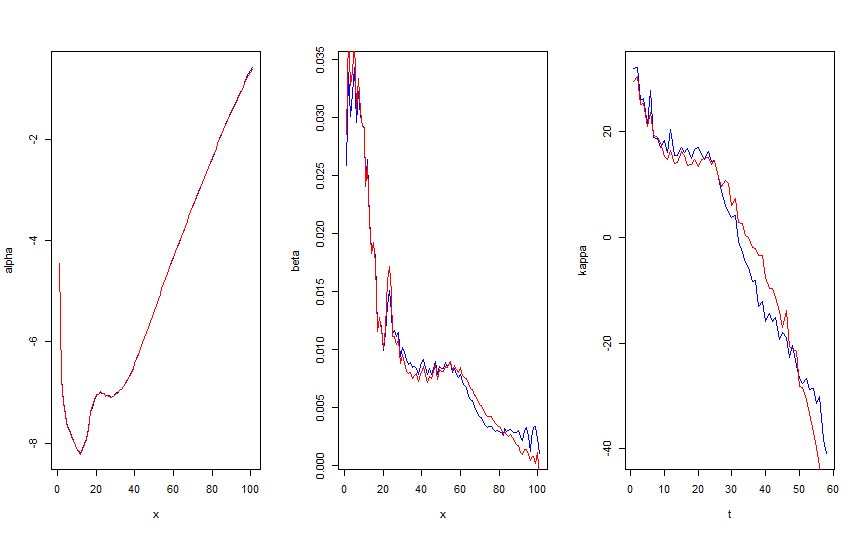
\includegraphics[scale=0.75]{NL3_Question7.png}
		
		\caption{Coefficients $\alpha_x, \beta_x, \kappa_t$ produced by gnm (red lines) and LC (blues lines) }
		\label{Figure_Question7}
		
	\end{figure}
\end{center}

\subsection*{Q8}
From equation (3) from the assignment we know that the relationship between $\alpha_x$ and $\mu_{xt}$ is given by $\mu_{xt} = \exp(\alpha_x + \beta_x \kappa_t)$. The increase from the log-mortality $\alpha_x$ (keeping all other parameters fixed) from $-8$ to $-7$ from age 16 to 18 implies that $\mu_{xt}$ increases by $\exp(1) \approx 2.72$. In the assignment about Gompertz and Makeham we have already seen this phenomenon and it is named the 'accident hump'.

\subsection*{Q9}
We execute the code and add one line to view the coefficients of the object \verb|g1|

\begin{verbatim}
> kappa.glm <- kappa.LC
> g1 <- glm(Dxt.vec ~ x*kappa.glm[t] + offset(lnExt.vec), poisson)
> c1 <- coef(g1)
> g1$deviance; g1$iter ## 27603.07 4
[1] 27603.07
[1] 4
> c1
\end{verbatim}

the output given from the call \verb|c1| is an intercept, \verb|x2| - \verb|x101| and \verb|kappa.glm[t]|,\verb|x2:kappa.glm[t]| - \verb|x101:kappa.glm[t]|. We can then retrieve the optimal parameter estimates by (using the intercept resp. \verb|kappa.glm[t]| as base contribution)

\begin{verbatim}
alpha.glm <- c(c1[1],c1[2:101]+c1[1])
beta.glm <- c(c1[102],c1[103:202]+c1[102])
\end{verbatim}

\subsection*{Q10}
We run the code as given in the assignment and obtain the following results

\begin{verbatim}
> g2 <- glm(Dxt.vec ~ 0 + x + t:beta.glm[x] + offset(lnExt.vec), poisson,
+           mustart=fitted(g1))
> c2 <- coef(g2)
> g2$deviance; g2$iter ## 23594.62 4
[1] 23594.62
[1] 4
> c2[c(1,nages,nages+1,nages+nyears-1,nages+nyears)] ## t58:beta.glm[x] is NA
x1            x101  t1:beta.glm[x] t57:beta.glm[x] t58:beta.glm[x] 
-6.0994748      -0.5598663      88.0965362       5.6195332              NA
\end{verbatim}

We see that the last coefficient \verb|t58:beta.glm[x]| is \verb|NA|. Using the command \verb|summary(g2)| we see that 1 coefficient is not defined because of singularities. Therefore the last coefficient is \verb|NA|. Since there is no base contribution (no constant in the regression) we can use the following to assign $\alpha_x$ and $\kappa_t$ (adding a zero for the parameter $\kappa_{58}$ because of the \verb|NA| result)

\begin{verbatim}
alpha.glm <- c2[1:101]
kappa.glm <- c(c2[102:158],0)
kappa.glm <- kappa.glm * sum(beta.glm)
beta.glm <- beta.glm/sum(beta.glm)
alpha.glm <- alpha.glm + mean(kappa.glm)*beta.glm
kappa.glm <- kappa.glm - mean(kappa.glm)
\end{verbatim}
where the transformations ensure we have the properties of Question 1.

\subsection*{Q11}

Using the inverse link function we can calculate \verb|fitted(g2)[532]| in terms of \verb|Ext.vec[532]|, \verb|alpha.glm[x[532]]|, \verb|beta.glm[x[532]]| and \verb
\verb|kappa.glm[t[532]])| as
\begin{verbatim}
exp(log(Ext.vec[532])+alpha.glm[x[532]]+beta.glm[x[532]]*kappa.glm[t[532]])
\end{verbatim} We check in \verb|R| if the two are equal by determining if the absolute value of the difference is small
and obtain the following output
\begin{verbatim}
> abs(exp(log(Ext.vec[532])+alpha.glm[x[532]]+
		beta.glm[x[532]]*kappa.glm[t[532]])-fitted(g2)[532])<0.001
x10 
TRUE
\end{verbatim}

which implies that the reconstruction and the value of \verb|fitted(g2)[532]| are equal (checked for a maximum difference of 0.0001).

\subsection*{Q12}

We execute the code from the assignment and obtain

\begin{verbatim}
> beta.glm <- beta.glm/sum(beta.glm)
> alpha.glm <- alpha.glm + mean(kappa.glm)*beta.glm
> kappa.glm <- kappa.glm - mean(kappa.glm)
> (d1 <- sum(dpois(Dxt.vec,Dxt.vec,log=TRUE))) ## -21643.76
[1] -21643.76
> (d2 <- sum(dpois(Dxt.vec,
+                  Ext.vec*exp(alpha.glm[x] + beta.glm[x] * kappa.glm[t]),
+                  log=TRUE))) ## -33441.07, same as d3
[1] -33441.07
> (d3 <- sum(dpois(Dxt.vec,fitted(g2),log=TRUE)))
[1] -33441.07
> (d4 <- log(prod(dpois(Dxt.vec,fitted(g2)))))## -Inf
[1] -Inf
> (d5 <- 2*sum(Dxt.vec*log(Dxt.vec/fitted(g2)) - (Dxt.vec-fitted(g2))))
[1] 23594.62
> (d1-d2)*2 ## 23594.62, same as d5
[1] 23594.62
\end{verbatim}

We see that the result \verb|d2| equals \verb|d3| and that \verb|d5| equals \verb|(d1-d2)*2 |. The results \verb|d2| and \verb|d3| are equal by construction (see Question 11). The result from \verb|d4| should be equal to the result from \verb|d3|. The difference is using the \verb|log=TRUE| option in \verb|d3| instead of taking the logarith from the products in \verb|d4|. The result in \verb|d4| is not equal because \verb|R| has difficulties in taking the logarithm of the very small probabilities. The equality of \verb|d5| and \verb|(d1-d2)*2| follows from MART (9.29). The calculation \verb|d5| is equal to right-hand side of MART (9.29) (with $\phi$ and $w_i$ equal to zero) and \verb|(d1-d2)*2| is equal to the middle expression of MART (9.29).

\subsection*{Q13}
We execute the code from the exercise and obtain the following result.

\begin{verbatim}
> range(tapply(Dxt.vec-fitted(g2),x,sum)) ## -3e-10 2e-10
[1] -3.885816e-10  2.038405e-10
> range(tapply(Dxt.vec-fitted(g2),t,sum)) ## -3300 2726
[1] -3299.962  2726.266
>
\end{verbatim}

The first line shows the range of the differences of the data versus the fit with respect to the ages $x$ and the second line shows the range of the differences of the data versus the fit with respect to the time $t$. The result shows that the residuals are very small with respect to the ages but can be significant with respect to time (residuals up between -3300 and 2726).


\subsection*{Q14}
We run the code from the assignment and obtain the given results
\begin{verbatim}
> kappa.glm <- kappa.LC
> oldDeviance <- 0; TotnIter <- 0; start=NULL
> system.time(
+   repeat
+   { g1 <- glm(Dxt.vec~x*kappa.glm[t]+offset(lnExt.vec), poisson, mustart=start)
+   c1 <- coef(g1)
+   alpha.glm <- c(c1[1],c1[2:101]+c1[1])
+   beta.glm <- c(c1[102],c1[103:202]+c1[102])
+   g2 <- glm(Dxt.vec ~ 0+x + t:beta.glm[x] + offset(lnExt.vec), poisson,
+             mustart=fitted(g1))
+   8
+   c2 <- coef(g2)
+   alpha.glm <- c2[1:101]
+   kappa.glm <- c(c2[102:158],0)
+   kappa.glm <- kappa.glm*sum(beta.glm); beta.glm <- beta.glm/sum(beta.glm);
+   alpha.glm <- alpha.glm + mean(kappa.glm)*beta.glm
+   kappa.glm <- kappa.glm - mean(kappa.glm)
+   TotnIter <- TotnIter + g1$iter + g2$iter
+   newDeviance <- g2$deviance;
+   done <- abs((oldDeviance-newDeviance)/newDeviance)<1e-6
+   cat(g1$deviance, "\t", g2$deviance, "\n")
+   oldDeviance <- newDeviance; start <- fitted(g2)
+   if (done) break
+   }
+ ) ## ~ 6 sec
27603.07 	 23594.62 
23416.47 	 23407.23 
23406.74 	 23406.71 
23406.71 	 23406.71 
user  system elapsed 
4.54    0.19    4.74 
> TotnIter ## 20
[1] 20
> 
> AIC(g1); AIC(g2) ## 67098.22 67010.22
[1] 67098.22
[1] 67010.22
> logLik(g1); logLik(g2) ## 'log Lik.' -33347.11 with df=202 and df=158
'log Lik.' -33347.11 (df=202)
'log Lik.' -33347.11 (df=158)
\end{verbatim}

The calculated log-likelihoods are equal for both models. Because not all parameters are determined in \verb|g1| and \verb|g2| the calculated AIC is not correct with respect to the complete model. Since the total effective number of paramters is $101+101+58 - 2 = 258$ (101 $\alpha_x$ parameters, 101 $\beta_x$ parameters, 58 $\kappa_t$ parameters and a redundancy of 2) the actual AIC calculation is equal to $AIC = -2 l + 2 k = -2 (-33347.11 - 258) = 67210.22$ which was obtain from the \verb|R| output 
\begin{verbatim}
> -2*(logLik(g1)-258)
'log Lik.' 67210.22 (df=202)
\end{verbatim}


\subsection*{Q15}

The $\mathbf{X}$ matrix has 5858 rows from the observations. For the \verb|g1| model we estimated the $\alpha_x$ and $\beta_x$ parameters so the matrix $\mathbf{X}$ has 202 columns. We check the dimensions of the matrix in \verb|R| and obtain the following output
\begin{verbatim}
> dim(model.matrix(g1))
[1] 5858  202
\end{verbatim} 
which are the dimensions we expected. Using the command given in the question we determine the amount of memory for each of the objects \verb|g1| and \verb|g2| and obtain
\begin{verbatim}
> object.size(g1); object.size(g2);
13254648 bytes
11130864 bytes
\end{verbatim}	
To determine which part of \verb|g1| occupies the most space we use the command given and obtain the following output
\begin{verbatim}
> sort(sapply(g1,object.size))
rank              deviance   aic            null.deviance iter   df.residual 
48                48         48             48            48         48 
df.null           converged  boundary       data          method     contrasts 
48                48         48             56            96         360 
control           formula    call           xlevels       terms      coefficients 
544               1720       1904           5952          6840       15408 
family            offset     effects        R             residuals  fitted.values 
45880             46904      105952         354080        375104     375104 
linear.predictors weights    prior.weights  y             model      qr 
375104            375104     375104         375104        603456     9811960 
\end{verbatim}
which shows that the \verb|qr| part of the object \verb|g1| occupies the most space.

\subsection*{Q16}

To find the parameters $\hat{b}$ and $\hat{c}$ that optimize the $\text{Gompertz}(b,c)$ likelihood we use a \verb|glm| call with offset \verb|offset(lnExt.vec)| and find the parameter values through exponentiating the estimates. The output of \verb|R| is the following for the complete estimate, the estimate restricted to the ages 30+ and the plots.
\begin{verbatim}
> x1 <- as.numeric(x)-1
> g3 <- glm(Dxt.vec ~ x1 + offset(lnExt.vec),poisson)
> g3$coefficients
(Intercept)          x1 
-9.11080428  0.08377865 
> 
> (b.Gompertz <- exp(coef(g3)[1]))
(Intercept) 
0.0001104658 
> (c.Gompertz <- exp(coef(g3)[2]))
x1 
1.087388 
> 
> alpha.Gompertz <- log(b.Gompertz)
> kappa.Gompertz <- log(c.Gompertz)
> beta.Gompertz <- (1:nages)-1
> 
> kappa.Gompertz <- kappa.Gompertz * sum(beta.Gompertz)
> beta.Gompertz <- beta.Gompertz/sum(beta.Gompertz)
> alpha.Gompertz <- alpha.Gompertz + mean(kappa.Gompertz)*beta.Gompertz
> kappa.Gompertz <- kappa.Gompertz - mean(kappa.Gompertz)
> 
> g3.30 <- glm(Dxt.vec ~ x1 + offset(lnExt.vec),poisson,subset = x1>=30)
> g3.30$coefficients
(Intercept)           x1 
-10.13570719   0.09782707 
>   
> (b.30.Gompertz <- exp(coef(g3.30)[1]))
(Intercept) 
3.96386e-05 
> (c.30.Gompertz <- exp(coef(g3.30)[2]))
x1 
1.102772 
> 
> alpha.30.Gompertz <- log(b.30.Gompertz)
> kappa.30.Gompertz <- log(c.30.Gompertz)
> beta.30.Gompertz <- (1:nages)-1
> kappa.30.Gompertz <- kappa.30.Gompertz * sum(beta.30.Gompertz)
> beta.30.Gompertz <- beta.30.Gompertz/sum(beta.30.Gompertz)
> alpha.30.Gompertz <- alpha.30.Gompertz + mean(kappa.30.Gompertz)*beta.30.Gompertz
> kappa.30.Gompertz <- kappa.30.Gompertz - mean(kappa.30.Gompertz)
> 
> par(mfrow=c(1,1))
> plot(alpha.LC,ylim=range(alpha.LC), ylab="alpha", xlab="x", col="blue", type="l")
> lines(alpha.Gompertz,col="black", type="l")
> lines(alpha.30.Gompertz,col="red", type="l")
>
\end{verbatim}
The parameter estimates on the complete set are
\begin{equation}
b = 1.104658 \times 10^{-4} \quad \text{and} \quad c = 1.087388 
\end{equation}
and the plot is given in Figure \ref{Figure_Question15}.

\begin{center}
	\begin{figure}[H]
		
		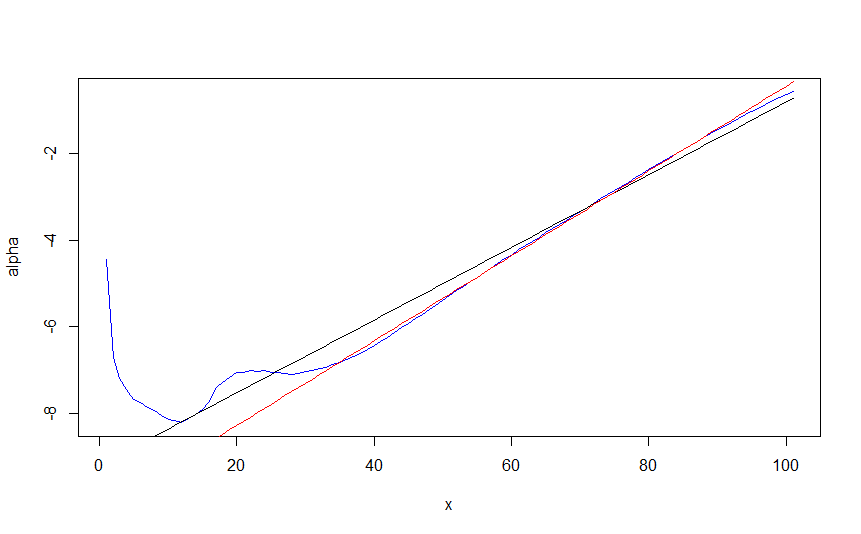
\includegraphics[scale=0.75]{NL3_Question16.png}
		
		\caption{Coefficient $\alpha_x$ estimated by LC (blue line),  Gompertz (black line) and Gompertz ages 30+ (red line) }
		\label{Figure_Question15}
		
	\end{figure}
\end{center}


\subsection*{Q17}
Using the code in the assignment we obtain the Figures from the assignment.

\begin{verbatim}
g4 <- glm(Dxt.vec~x1*t-x1-1+offset(lnExt.vec), poisson, subset=x1>=30)
b <- 1e5*exp(head(coef(g4),nyears)); c <- 100*(exp(tail(coef(g4),nyears))-1)
par(mfrow=c(1,2))
plot(b, xlab="t", ylab="b*100000", ylim=c(0,10), type="l", yaxp=c(0,10,2),
main="Gompertz parameters b;\nages 30+")
plot(c, xlab="t", ylab="c-1 in %", ylim=c(9,12), type="l",
yaxp=c(9,12,3), main="Gompertz parameters c")
\end{verbatim}

To extrapolate the trend in the graph of $b_t$ and determine the time $t$ for which $b_t = 0$ we use regression of $b_t$ against $t$ and solve for $b_t = 0$ in \verb|R|. We have the following output
\begin{verbatim}
> t1 <- 1:nyears
> b.lm <- lm(b~t1,subset = t1>20)
> b.lm$coefficients
(Intercept)          t1 
9.6359275  -0.1411485 
> 
> t.intersect <- -b.lm$coefficients[1]/b.lm$coefficients[2]
> t.intersect
(Intercept) 
68.26802 
>
\end{verbatim}
At time $t=68.27$ we have that $b_t = 0$. A negative $b_t$ implies that there is a negative mortality rate and no people will be dying.

\subsection*{Q18}

Using the following code:
\begin{verbatim}
b <- b/1e5; c<- c/100 + 1;
log.mortality <-function(x){ log(b) + 	x * log(c)}

plot(log.mortality(65), xlab="t", ylab="Log-mortality", type="l",col="black",ylim=c(-5,0))
lines(log.mortality(75), col="red",  type="l")
lines(log.mortality(85), col="blue", type="l")
\end{verbatim}

we obtain Figure \ref{Figure_Question18}. There is a shift of the curve upwards for higher ages and for values of $t$ larger then 30 the log-mortality is descending with $t$.

\begin{center}
	\begin{figure}[H]
		
		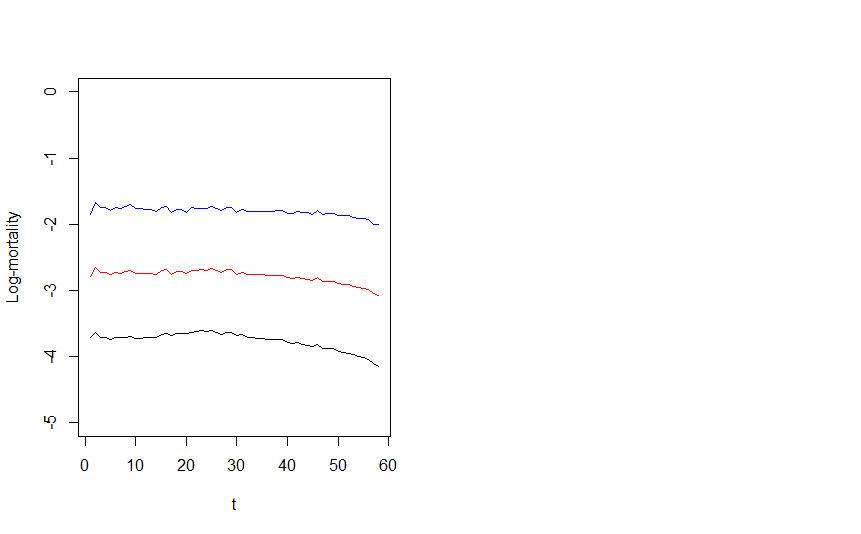
\includegraphics[scale=0.60]{NL3_Question18.png}
		
		\caption{Log-mortality for ages 65 (black line), 75 (red line) and 85 (blue line)}
		\label{Figure_Question18}
		
	\end{figure}
\end{center}


\section{Analyzing a bonus-malus system using GLM}

\subsection*{Q1}

\subsubsection*{a)}
We are asked to check if the values in Table 9.8 from MART are correct. For this, we first run the code given in the exercise:

\begin{verbatim}
> rm(list=ls(all=TRUE)) ## First remove traces of previous sessions
> fn <- "http://www1.fee.uva.nl/ke/act/people/kaas/Cars.txt"
> Cars <- read.table(fn, header=TRUE)
> Bminus1 <- Cars$B - 1; Bis14 <- as.numeric(Cars$B==14)
> Cars$A <- as.factor(Cars$A); Cars$R <- as.factor(Cars$R)
> Cars$M <- as.factor(Cars$M); Cars$U <- as.factor(Cars$U)
> Cars$B <- as.factor(Cars$B); Cars$WW <- as.factor(Cars$WW)
> ActualWt <- c(650,750,825,875,925,975,1025,1075,1175,1375,1600)
> W <- log(ActualWt/650)[Cars$WW]
> 
> # GLM analysis
> 
> g1 <- glm(TotCl/Expo~R+A+U+W+Bminus1+Bis14, quasipoisson, wei=Expo, data=Cars)
> g2 <- glm(TotCl/Expo~R+A+U+W+Bminus1+Bis14+M, quasipoisson, wei=Expo, data=Cars)
> g3 <- glm(TotCl/Expo~R+A+U+W+B, quasipoisson, wei=Expo, data=Cars)
> 
> anova(g1,g2)
Analysis of Deviance Table

Model 1: TotCl/Expo ~ R + A + U + W + Bminus1 + Bis14
Model 2: TotCl/Expo ~ R + A + U + W + Bminus1 + Bis14 + M
  Resid. Df Resid. Dev Df Deviance
1      7515   38616941            
2      7513   38614965  2   1975.8
> anova(g1,g3)
Analysis of Deviance Table

Model 1: TotCl/Expo ~ R + A + U + W + Bminus1 + Bis14
Model 2: TotCl/Expo ~ R + A + U + W + B
  Resid. Df Resid. Dev Df Deviance
1      7515   38616941            
2      7504   38544506 11    72435
> 
> # Multiplicative coefficients
> options(digits=7)
> exp(coef(g1)); exp(coef(g2)); exp(coef(g3))
(Intercept)          R2          R3          A2          A3          U2           W
524.3016583   1.0842682   1.1916130   0.4147224   0.6184468   1.3841303   2.3722083
    Bminus1       Bis14 
  0.8978647   1.1053665 
(Intercept)          R2          R3          A2          A3          U2           W 
522.6627527   1.0842767   1.1914111   0.4147232   0.6184538   1.3835062   2.3721668 
    Bminus1       Bis14          M2          M3 
  0.8978640   1.1053568   1.0073260   1.0014581   
(Intercept)          R2          R3          A2          A3          U2           W 
515.5320549   1.0843018   1.1916593   0.4143437   0.6178700   1.3841612   2.3722369
         B2          B3          B4          B5          B6          B7          B8 
  0.9111279   0.8275175   0.7403718   0.6842609   0.6088526   0.5416103   0.4489065 
         B9         B10         B11         B12         B13         B14 
  0.4151901   0.3888576   0.3459030   0.3143452   0.2832722   0.2773037 
\end{verbatim}

All coefficients can be checked individually against table 9.8 and are the same, except for models \verb|g1| and \verb|g2|, because the bonus malus risk factor is taken as numeric. This means that the factors in the table have been calculated from the factor for $B2$ to the power $B - 1$. The coefficient for \verb|Bminus1| differs only in the 7th decimal spot and the table is given with 4 decimals. This means that if we only need to check one of the two models. We do this by recalculating the values in \verb|R|.

\begin{verbatim}
> bm_class <- seq(1,13,1)
> bm_coef <- exp((bm_class-1)*coef(g1)["Bminus1"])
> bm_coef
[1] 1.0000000 0.8978647 0.8061610 0.7238236 0.6498956 0.5835184 0.5239205
[8] 0.4704098 0.4223643 0.3792260 0.3404937 0.3057173 0.2744927
\end{verbatim}

These values also correspond with those in table 9.8

\subsubsection*{b)}
Using the coefficients of \verb|g1|, \verb|g2| and \verb|g3|, compute the fitted values for the cell 4000.

For this, we use the coefficients in \verb|R|. Recalculating these by hand would be rather pointless and is an exercise in working neatly over understanding the subject matter.

\begin{verbatim}
> # Observed value
> g1$y[4000]
4000 
326.4545 
> 
> # Fitted value
> fitted(g1)[4000]; fitted(g2)[4000]; fitted(g3)[4000]
4000 
634.0642 
4000 
636.416 
4000 
644.5283 
\end{verbatim}

What we can see is the all three GLM's have a fitted value that is about twice as large as the actual value. Not one of the models is close to the observed value, but the models are quite close together in their estimate.

\subsubsection*{c)}

We now explain the result of the following \verb|R|-code.

\begin{verbatim}
> g2$family$linkinv(model.matrix(g2)[4000,]%*%coef(g2))
        [,1]
[1,] 636.416
\end{verbatim}

This result is equal to the fitted value of the \verb|g2| model. This is no surprise, considering the code is equal to the definition of the fitted value for cell 4000. The inner product of the values of the risk factors and their corresponding coefficients gives the linear estimator for that cell, after which the \verb|linkinv| function is applied, which is the exponential function. This results in the fitted value.

\subsection*{Q2}

First we will determine the scale factor $\phi$ using a 'rich' model, meaning that the values of both the weight of the car and the BM class are used as factors.

\begin{verbatim}
> g.rich <- glm(TotCl/Expo~R+A+U+WW+B, quasipoisson, wei=Expo, data=Cars)
> anova(g.rich)
Analysis of Deviance Table

Model: quasipoisson, link: log

Response: TotCl/Expo

Terms added sequentially (first to last)


     Df Deviance Resid. Df Resid. Dev
NULL                  7523  116167018
R     2  2586478      7521  113580540
A     2 23288859      7519   90291681
U     1  4479946      7518   85811735
WW   10  6931993      7508   78879742
B    13 40358336      7495   38521406
\end{verbatim}

We determine the scale factor to be $\frac{38521406}{7495} = 5139.61$. Or in \verb|R|:

\begin{verbatim}
> phi <- 38521406/7495
\end{verbatim}

To check whether \verb|Bis14| can be removed from the model, we use an \verb|anova| call on the model with \verb|Bis14| (\verb|g1|) and without (\verb|g.test|).

\begin{verbatim}
> g.test <- glm(TotCl/Expo~R+A+U+W+Bminus1, quasipoisson, wei=Expo, data=Cars)
> anova(g.test,g1)
Analysis of Deviance Table

Model 1: TotCl/Expo ~ R + A + U + W + Bminus1
Model 2: TotCl/Expo ~ R + A + U + W + Bminus1 + Bis14
  Resid. Df Resid. Dev Df Deviance
1      7516   38755743            
2      7515   38616941  1   138802
\end{verbatim} 

Next we test if the inclusion of \verb|Bis14| is significant:

\begin{verbatim}
> test <- function (Df, Deviance){
+   scaled.dev <- Deviance/phi
+   test.dev <- qchisq(0.95,Df)
+   return(scaled.dev>test.dev)
+ }
> test(1, 138802)
[1] TRUE
\end{verbatim}

First we calculate the scaled deviance. Then we calculate the 95-th percentile of the $\chi^{2}(k)$ distribution with \verb|Df| degrees of freedom. When the improvement of scaled deviance is larger than the test value, the increase is significant. The test is implemented as a function, so it can be reused in the rest of the exercise. Also the test returns \verb|TRUE|, therefore the inclusion of \verb|Bis14| is a significant improvement of the model and can not be removed.

Then we check if \verb|B| can be removed from model \verb|g3|.

\begin{verbatim}
> g.test <- glm(TotCl/Expo~R+A+U+W, quasipoisson, wei=Expo, data=Cars)
> anova(g.test,g3)
Analysis of Deviance Table

Model 1: TotCl/Expo ~ R + A + U + W
Model 2: TotCl/Expo ~ R + A + U + W + B
  Resid. Df Resid. Dev Df Deviance
1      7517   78902891            
2      7504   38544506 13 40358385
> test(13,40358385)
[1] TRUE
\end{verbatim}

The test value is \verb|TRUE|, so \verb|B| can not be removed from the model. Next we check whether \verb|W| can be removed from the model:

\begin{verbatim}
> g.test <- glm(TotCl/Expo~R+A+U+B, quasipoisson, wei=Expo, data=Cars)
> anova(g.test,g3)
Analysis of Deviance Table

Model 1: TotCl/Expo ~ R + A + U + B
Model 2: TotCl/Expo ~ R + A + U + W + B
  Resid. Df Resid. Dev Df Deviance
1      7505   45495122            
2      7504   38544506  1  6950616
> test(1,6950616)
[1] TRUE
\end{verbatim}

This result implies that \verb|W| can not be removed from the model \verb|g3|.

Is it helpful to allow separate coefficients for the weight class in model \verb|g1|. We again check using the \verb|anova| and \verb|test| functions.

\begin{verbatim}
> g.test <- glm(TotCl/Expo~R+A+U+WW+Bminus1+Bis14, quasipoisson, wei=Expo, data=Cars)
> anova(g1, g.test)
Analysis of Deviance Table

Model 1: TotCl/Expo ~ R + A + U + W + Bminus1 + Bis14
Model 2: TotCl/Expo ~ R + A + U + WW + Bminus1 + Bis14
  Resid. Df Resid. Dev Df Deviance
1      7515   38616941            
2      7506   38593888  9    23053
> test(9,23053)
[1] FALSE
\end{verbatim}

This shows that allowing separate coefficients for the weight classes would not be an improvement.

\subsection*{Q3}

To answer this question, we run the \verb|test| function defined earlier:

\begin{verbatim}
> test(7515-7491,38616941-38408588)
[1] TRUE
\end{verbatim}

The interaction terms do improve the model significantly. It might be worthwhile to investigate which interaction terms give the most improvement, because there might be some interaction terms which are not significant by themselves.

\subsection*{Q4}

First we estimate the number of claims and the size per claim as described. We can combine the two models by adding their coefficients, because directly combining the two models will give a product of two exponentials, which is the same as one exponential with the arguments summed. We compare the resulting coefficients with a direct estimation.

\begin{verbatim}
> g.nCl <- glm(nCl/Expo~R+A+U+W+Bminus1+Bis14, quasipoisson, wei=Expo, data=Cars)
> g.sCl <- glm(TotCl/nCl~R+A+U+W+Bminus1+Bis14, Gamma(link="log"), wei=nCl, data=Cars)
> g.direct <- glm(TotCl/Expo~R+A+U+W+Bminus1+Bis14, quasipoisson, wei=Expo, data=Cars)
> 
> mult.coef <- exp(coef(g.nCl)+coef(g.sCl))
> direct.coef <- exp(coef(g.direct))
> mult.coef; direct.coef
(Intercept)          R2          R3          A2          A3          U2 
525.1107841   1.0856608   1.1901279   0.4134531   0.6145069   1.3823142 
          W     Bminus1       Bis14 
  2.3827096   0.8979376   1.1057074 
(Intercept)          R2          R3          A2          A3          U2 
524.3016583   1.0842682   1.1916130   0.4147224   0.6184468   1.3841303 
          W     Bminus1       Bis14 
  2.3722083   0.8978647   1.1053665 
\end{verbatim}

The resulting models have very similar results and attribute about the same amount of risk to each risk factor.

\end{document}
